% Auriga theme
% https://github.com/anishathalye/auriga

\documentclass[14pt,aspectratio=169]{beamer}
\usepackage{pgfpages}
\usepackage{fancyvrb}
\usepackage{booktabs,dcolumn}
\usepackage{tikz}
\usetikzlibrary{arrows.meta, positioning, quotes}
\usepackage{pgfplots}

% \ifnotes
% \setbeamertemplate{note page}[plain]
% \setbeameroption{show notes on second screen=right}
% \fi

\usetheme{auriga}
\usecolortheme{auriga}

% define some colors for a consistent theme across slides
\definecolor{red}{RGB}{181, 23, 0}
\definecolor{blue}{RGB}{0, 118, 186}
\definecolor{gray}{RGB}{146, 146, 146}

\title{Historia Económica Argentina}

\author{\underline{Sebastián Freille} \inst{1}}

\institute[shortinst]{\inst{1} IEF-UNC \\ UCC}
\date{}

\AtBeginSection[]{
    \begin{frame}
    \vfill
    \centering
    \begin{beamercolorbox}[sep=8pt,center,shadow=true,rounded=true]{title}
        \usebeamerfont{title}\insertsectionhead\par%
    \end{beamercolorbox}
    \vfill
    \end{frame}
}



\AtBeginSubsection[]{
    \begin{frame}
    \vfill
    \centering
    \begin{beamercolorbox}[sep=6pt,center,shadow=true,rounded=true]{title}
        \usebeamerfont{title}\insertsubsectionhead\par%
    \end{beamercolorbox}
    \vfill
    \end{frame}
}


\AtBeginSubsubsection[]{
    \begin{frame}
    \vfill
    \centering
    \begin{beamercolorbox}[sep=4pt,center,shadow=true,rounded=true]{title}
        \usebeamerfont{title}\insertsubsubsectionhead\par%
    \end{beamercolorbox}
    \vfill
    \end{frame}
}


\begin{document}

{
  % rather than use the frame options [noframenumbering,plain], we make the
  % color match, so that the indicated page numbers match PDF page numbers
  \setbeamercolor{page number in head/foot}{fg=background canvas.bg}
  \begin{frame}
    \titlepage
  \end{frame}
}

  
  \section{Capítulo 3. La Economía Política del Peronismo, 1946-1955}


  \section{Resumen 1946-1948}
  

 \begin{frame}\frametitle{Medidas y efectos}
    \begin{itemize}\itemsep 10pt
      \item Las medidas aplicadas durante los años excepcionales de
        1946 a 1948 fueron de corte keynesiano convencional
        $\longrightarrow$ crédito subsidiado a la inversión, aumentos
        salariales y expansión del gasto público (y déficit
        fiscal). Políticas orientadas al corto plazo (recuperación
        económica) más que al crecimiento de largo plazo
        \item Consecuencias no deseadas de estas políticas
          $\longrightarrow$ aumento de la tasa de inflación y del
          impuesto inflacionario, caída en los depósitos a plazo,
          déficit comercial y un aumento en la prima del dólar en
          mercado paralelo. 
                 \end{itemize}
               \end{frame}


                \begin{frame}\frametitle{Medidas y efectos (cont.)}
    \begin{itemize}\itemsep 10pt
      \item Es importante no desconocer que las autoridades conocían
        los costos de una política redistributiva y
        mercadointernista. ¿Por qué la siguieron entonces?
        \begin{itemize}\itemsep 5pt \medskip
        \item porque era el sustento de la \textbf{consolidación
            política} de la nueva fuerza entre los trabajadores
          \item porque la expectativa de abrir la economía ante un
            inminente (según Perón)
            \textbf{nuevo conflicto mundial} no tenía sentido 
          \end{itemize}
          \item Es así como durante este período la política económica
            se subordinó a dos objetivos bien claros: fuerte
            redistribución de ingresos hacia trabajadores urbanos y
            aumento de la actividad estatal
                 \end{itemize}
               \end{frame}


                               \begin{frame}\frametitle{Medidas y efectos (cont.)}
                                 \begin{block}{Ilusión monetaria e
                                     impuesto inflacionario}
                                   Varios autores consideran que gran
                                   parte del \textit{rationale} de la
                                   política económica del peronismo en
                                   el primer período puede ser
                                   explicada por la presencia de
                                   \textit{ilusión monetaria} entre
                                   los ciudadanos. Evidencia de ello
                                   es que los depositantes
                                   (ahorradores netos) reaccionaron
                                   lenta y tardíamente a la erosión
                                   de sus ahorros en términos reales
                                   --transferencia de ingresos desde
                                   ahorradores netos (campo, clase media) a desahorradores
                                   netos (industria). Esto es, al
                                   menos en comparación con períodos
                                   posteriores (1959, 1975, 1982-83) en que la ilusión
                                   monetaria tenía corta vida. 
                                   \end{block}
               \end{frame}
      
      

 \section{Crisis y cambio}

 \begin{frame}\frametitle{Crisis de 1949}
  \begin{itemize}\itemsep 10pt
      \item La reversión de la balanza comercial en 1949 y la
        aceleración de la inflación empezaron a mostrar las primeras
        grietas del modelo $\longrightarrow$ luego consolidados en dos
        problemas de largo plazo --\textbf{inflación} y
        \textbf{stop-and-go}
        \item Caída en TIE (¿vuelta a la normalidad de tendencia
          decreciente?) y también caida en cantidades
          \item Se suma un primera fuerte sequía de la campaña 1949/50
            $\longrightarrow$ exportó casi la mitad en valor que el
            año 1948
                 \end{itemize}
               \end{frame}


 
  \begin{frame}\frametitle{Crisis de 1949 (cont.)}
\begin{figure}[hxtbp]\vspace{0cm}
  \centering
  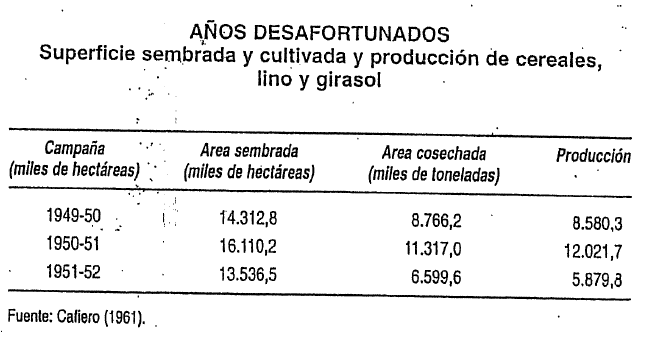
\includegraphics[scale=0.75]{uni3_crisis01}
   \label{fig:uni1_01}
\end{figure} 
  \end{frame}
      

  \begin{frame}\frametitle{Crisis de 1949 (cont.)}
  \begin{itemize}\itemsep 10pt
      \item Esta situación hizo que la escasez de divisas generara
        cuellos de botella importantes en los sectores que dependían
        de M para su producción (industria)
      \item Intensificación de controles cambiarios y permisos de M
        \item La situación de la industria se agravó con la
          desaceleración del crédito hacia ella
          \item Hubo algunos intentos para moderar el crecimiento de
            la cantidad de dinero
                 \end{itemize}
               \end{frame}



  \begin{frame}\frametitle{Crisis y cambio}
  \begin{itemize}\itemsep 10pt
      \item Reemplazo del equipo económico trajo una señal de orden
        y prudencia $\longrightarrow$ viraje hacia política más
        conservadora en algunas dimensiones:
        \begin{itemize}\itemsep 5pt \medskip
        \item deseo de integración a la economía global
        \item incentivos a la producción agropecuaria
          \item mayor racionalidad del crédito productivo
          \end{itemize}
          \item No obstante, en otras dimensiones, continuó la misma
            orientación $\longrightarrow$ política económica basada en
            nociones e ideas de igualdad
                 \end{itemize}
               \end{frame}


                \begin{frame}\frametitle{Primera etapa: 1949-50}
  \begin{itemize}\itemsep 10pt
      \item Se limitó la expansión del sector público en la economía
        aunque se buscó mantener el salario real alto
        \item Disminuyó mucho el crédito al sector publico y algo al
          sector privado
          \item Durante estos años de crisis, la política económica
            del peronismo estuvo en la disyuntiva entre cambio y
            continuidad (a pesar de que por razones obvias la
            continuidad era imposible)
                 \end{itemize}
               \end{frame}



  \begin{frame}\frametitle{Primera etapa: 1949-50 (cont.)}
\begin{figure}[hxtbp]\vspace{0cm}
  \centering
  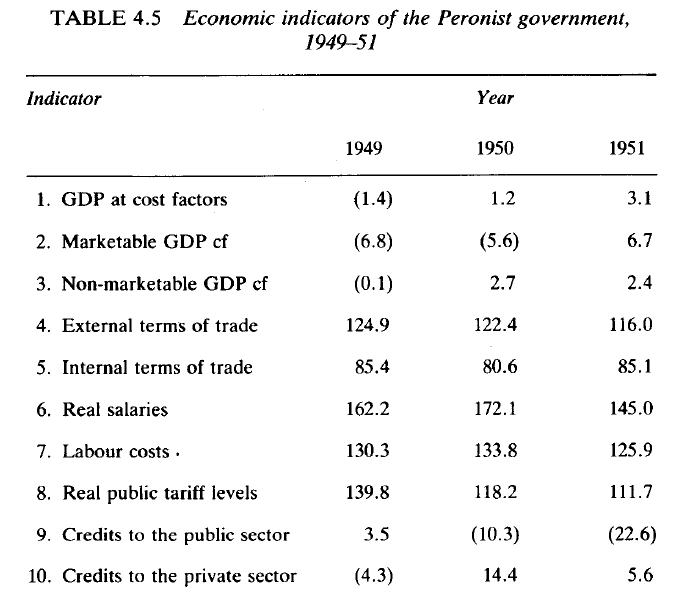
\includegraphics[scale=0.65]{uni3_crisis02}
   \label{fig:uni1_01}
\end{figure} 
  \end{frame}


\begin{frame}\frametitle{Primera etapa: 1949-50 (cont.)}
\begin{figure}[hxtbp]\vspace{0cm}
  \centering
  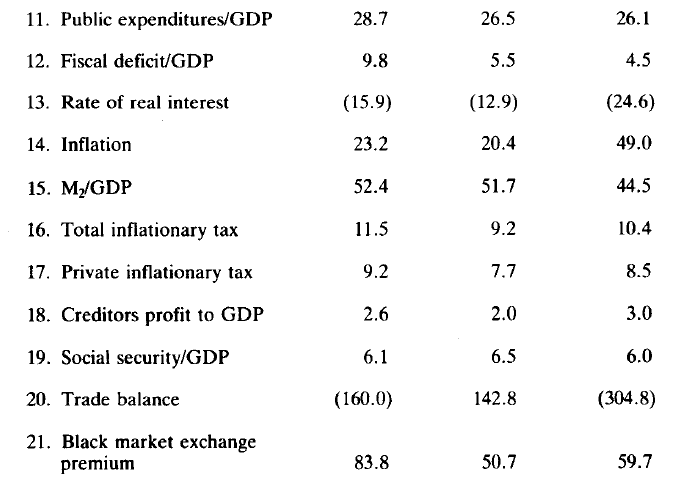
\includegraphics[scale=0.65]{uni3_crisis03}
   \label{fig:uni1_01}
\end{figure} 
  \end{frame}
  

               
                  \begin{frame}\frametitle{Primera etapa: 1949-50 (cont.)}
  \begin{itemize}\itemsep 10pt
      \item Un problema en esta crisis fue que el gobierno no pudo/no
        supo tomar medidas para contrarrestar los acontecimientos
        externos $\longrightarrow$ acentuación de sesgo
        anti-exportador ($\frac{P_{T}}{P_{NT}}$), crédito aun enfocado
        a sectores no transables
        \item Era necesario avanzar en una \textit{des-politización}
          de las decisiones de política económica
          \item En 1949, cae la producción industrial y recién en 1950
            el sector agropecuario empezó a recibir crédito comercial
                 \end{itemize}
               \end{frame}


               
                  \begin{frame}\frametitle{Primera etapa: 1949-50 (cont.)}
  \begin{itemize}\itemsep 10pt
      \item La idea de empezar a abrir la economía hacia el mercado
        externo surge tímida inicialmente y con cautela
        $\longrightarrow$ luego de 3 años de la guerra y hacia 1950,
        países europeos creciendo a nivels pre-guerra. Mas
        competidores y eventual temor por entrada de manufacturas
        externas
        \item En lo monetario, monetización ($M2/GDP$) había bajado de
          manera significativa (retiro de depósitos a plazo), la
          brecha del tipo de cambio paralelo/oficial llegó al 60\%
          \item El balance comercial negativo más alto desde 1946. 
                 \end{itemize}
               \end{frame}


 \begin{frame}\frametitle{Segunda etapa: 1951-55}
  \begin{itemize}\itemsep 10pt
      \item La prioridad era evitar un colapso económico --1949 en
        este sentido implicó un cambio de rumbo hacia mayores
        incentivos a la producción de transables
        \item Consecuencia $\longrightarrow$ caída de producción
          industrial y de salarios reales (hasta un 25\%) en 1952 y
          1953.
          \item Ejemplo (¿primero?) de la habilidad de usar política
            económica activa para estabilizar la economía luego de crisis
                 \end{itemize}
               \end{frame}



               \begin{frame}\frametitle{Segunda etapa: 1951-55}
  \begin{itemize}\itemsep 10pt
      \item Hay dos aspectos salientes de la política económica entre
        1952 y 1955:
        \begin{itemize}\itemsep 5pt \medskip
        \item Incentivos a producción de transables $\longrightarrow$
          operados no a través del sistema de precios sino a través de
          subsidios/créditos
          \item Gradual cambio de actitud en el gobierno peronista en
            relación a la inserción del país en el flujo de comercio internacional
          \end{itemize}
          \item Estos dos aspectos contextualizan gran parte de las
            medidas adoptas y decisiones tomadas como parte de este
            ``viraje conservador'' en la política económica peronista
                 \end{itemize}
               \end{frame}
               

\begin{frame}\frametitle{Segunda etapa: 1951-55 (cont.)}
\begin{figure}[hxtbp]\vspace{0cm}
  \centering
  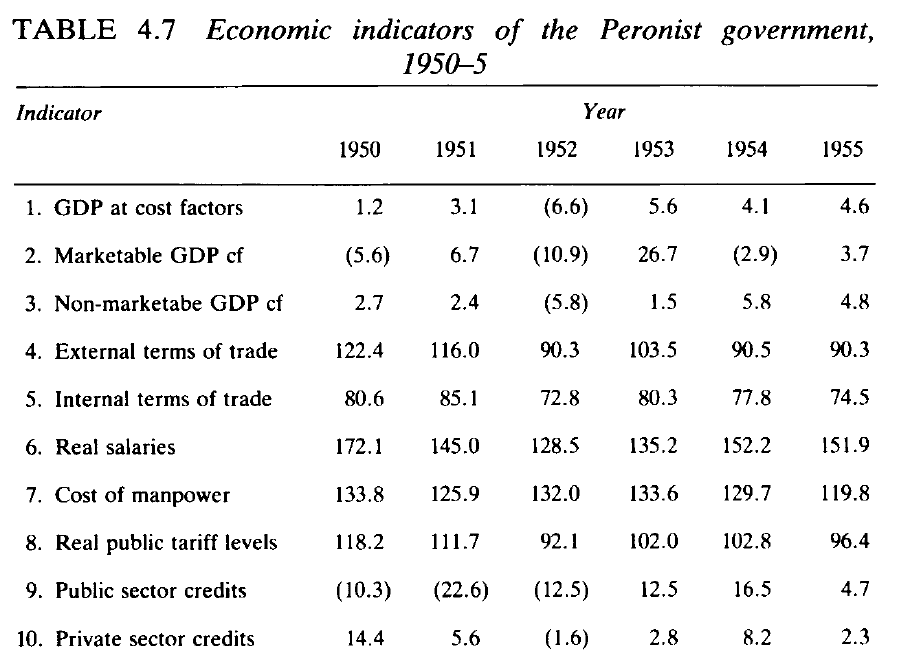
\includegraphics[scale=0.65]{uni3_crisis04}
   \label{fig:uni1_01}
\end{figure} 
  \end{frame}



\begin{frame}\frametitle{Segunda etapa: 1951-55 (cont.)}
\begin{figure}[hxtbp]\vspace{0cm}
  \centering
  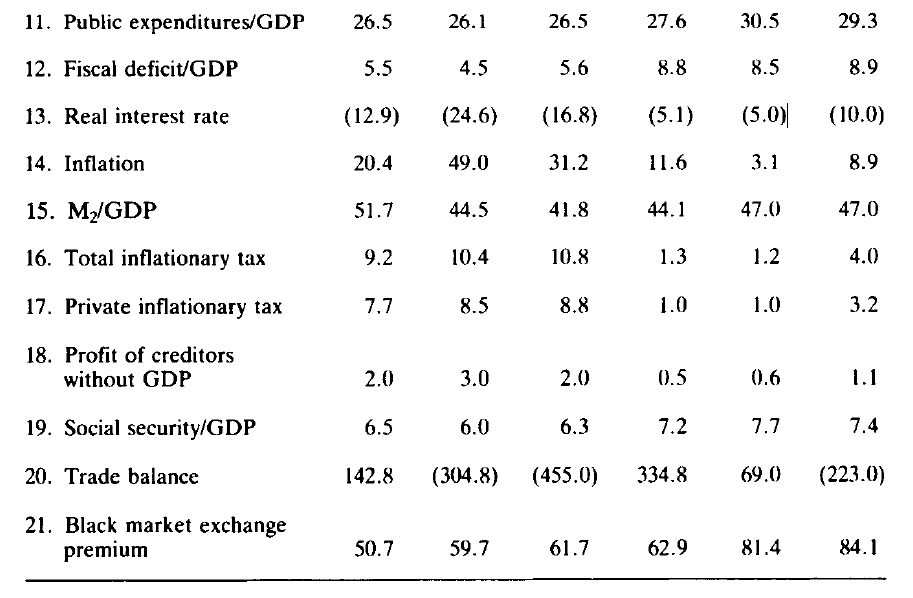
\includegraphics[scale=0.65]{uni3_crisis05}
   \label{fig:uni1_01}
\end{figure} 
  \end{frame}



       \begin{frame}\frametitle{Segunda etapa: 1951-55 (cont.)}
  \begin{itemize}\itemsep 10pt
      \item Los precios relativos agro/industria declinaron durante
        1952-55 pero el crédito al sector agropecuario creció de 11\%
        al 31\% en 1950-55
        \item Las distorsiones sin embargo existieron
          $\longrightarrow$ sobrevaluación del peso
          \item Se reconocía que la sobrevaluación del peso era un
            problema pero que para ello se debía atacar las causas de
            la inflación
            \item Medidas transitorias --reducciones impositivas,
              facilidades de crédito y cargos especiales de
              transporte- hasta que corrigiera tipo de cambio
                 \end{itemize}
               \end{frame}
               

   \begin{frame}\frametitle{Segunda etapa: 1951-55 (cont.)}
  \begin{itemize}\itemsep 10pt
      \item El segundo elemento --idea sobre integración a la economía
        mundial- siempre estuvo detrás de la actitud cautelosa de la
        administración peronista
        \item El cambio de actitud apareció luego de la guerra de
          Corea --conflictos futuros localizados y no mundiales .Aún
          así, era necesario llevar a cabo una fuerte devaluación.
          \item Hacia 1953, era claro que el gobierno tenía
            preocupación sobre (la falta de) una estrategia de largo plazo
                 \end{itemize}
               \end{frame}
               


                  \begin{frame}\frametitle{Segunda etapa: 1951-55 (cont.)}
  \begin{itemize}\itemsep 10pt
      \item Cada vez más países relajaban sus controles de cambios y
        había excedentes de capital importantes $\longrightarrow$
        posibilidad de inversión extranjera directa (IED)
      \item El gobierno promovió tipos de cambios diferenciales
        $\longrightarrow$ el más alto para estimular nuevas
        exportaciones industriales
        \item Las medidas no fueron efectivas en el corto plazo
          --recién hacia 1955 las manufacturas alcanzaron 4\% del
          total exportado
                 \end{itemize}
               \end{frame}
               

  \begin{frame}\frametitle{Segunda etapa: 1951-55 (cont.)}
  \begin{itemize}\itemsep 10pt
      \item Junto a estas medidas, se siguió un programa de austeridad
        (luego de pasadas las elecciones) --sin perder apoyo de
        trabajadores. ¿Golpe del 1955 por razones económicas?
        \item PBI había crecido al 5\% en 1953-55 y 4\% en
          1956-58. Incremento de establecimientos industriales de 85
          mil a 148 mil entre 1946-55.
          \item Tasa de inflación en 1953-55 la más baja del regimen
            --al momento de su caída, las tasas de inflación estaban
            cayendo (PBI y salarios creciendo)           
                 \end{itemize}
               \end{frame}


  \begin{frame}\frametitle{Segunda etapa: 1951-55 (cont.)}
  \begin{itemize}\itemsep 10pt
      \item Reducción del impuesto inflacionario en 1953-55
        $\longrightarrow$ remonetización (de 41 a 47). Tasas de
        interés positivas aunque bajas
        \item Retornó algo de la confianza (mayores depositos y
          ahorros)
          \item Recuperación parcial de salario real en 1953-55 (pero
            a niveles mas bajos que 1950) $\longrightarrow$ gradual
            baja del costo laboral por aumentos de productividad
                 \end{itemize}
               \end{frame}
               


  \begin{frame}\frametitle{Segunda etapa: 1951-55 (cont.)}
    \begin{block}{Evaluación de Prebisch}
        Argentina está atravesando la mayor crisis en su desarrollo
        económico; mayor que bajo el Presidente Avellaneda y mayor que
        aquella de los 1890s y la de 25 años atrás en medio de la
        Depresión Mundial. El país en aquellos momentos aún tenía las
        fuerzas productivas intactas. Este no es el caso ahora: los
        factores dinámicos de su economía han sido seriamente
        afectados y un esfuerzo intenso y persistente será necesario
        para reestablecer el ritmo vigoroso de desarrollo
        \end{block}
               \end{frame}


                 \begin{frame}\frametitle{Segunda etapa: 1951-55 (cont.)}
  \begin{itemize}\itemsep 10pt
      \item ¿Es justificada la visión negativa de Prebisch? Si uno
        toma la perspectiva de corto plazo, probablemente no. Si uno
        piensa en una perspectiva de largo plazo, si es más razonable
        \item La administración peronista a través de sus dos períodos
          de crecimiento, 1946-1948 y 1953-55 (menor), se basó
          esencialmente en el crecimiento del gasto público y los
          déficits fiscales.
          \item Existió durante todo este período una muy baja tasa de
            acumulación y formación de K que impactó en la inversión
            privada --local como extranjera. 
                 \end{itemize}
               \end{frame}


     \begin{frame}\frametitle{Resumen de los dos gobiernos: 1946-1955}
  \begin{itemize}\itemsep 10pt
      \item El peronismo priorizó un claro objetivo $\longrightarrow$
        distribución del Y en favor de obreros industriales [lógica
        política: movimiento político y base social]
        \item El peronismo utilizó al Estado como motor e instrumento
          al servicio de aquel objetivo --ya sea como control o
          intervención [lógica filosofía política: noción
          centralizadora --cambiaría en 1949] 
                 \end{itemize}
               \end{frame}


                \begin{frame}\frametitle{Resumen de los dos gobiernos:
                    1946-1955 (cont.)}
  \begin{itemize}\itemsep 10pt
      \item Las principales politicas para lograr el objetivo
        influyeron más a través de créditos/subsidios que a través del
        sistema de precios relativos
        \item Para hacer crecer el gasto público, utilizó
          alternativamente diferentes instrumentos $\longrightarrow$
          aumentó impuestos a sectores de negocios y clase media; ``creó''
          el impuesto inflacionario (10\% del PBI)
                 \end{itemize}
               \end{frame}


 \begin{frame}\frametitle{Resumen de los dos gobiernos:
                    1946-1955 (cont.)}
  \begin{itemize}\itemsep 10pt
      \item Se usó al déficit fiscal en momentos de expansión y de
        recesión (política pro-cíclica) $\longrightarrow$ crédito era
        barato y disponible por ahorro forzozo
        \item No se siguió una estrategia de desarrollo de largo plazo
          $\longrightarrow$ aumentos de W y de gast público en
          1946-48; aún cuando luego fue más austero, persistió la
          sobrevaluacíon de moneda local (perjudicó estrategia de
          promocíon de X y sustitución de M)
                 \end{itemize}
               \end{frame}


\begin{frame}\frametitle{Resumen de los dos gobiernos:
                    1946-1955 (cont.)}
  \begin{itemize}\itemsep 10pt
      \item La ``solución'' al problema de la sobrevaluación no
        vendría a través de sistema de precios relativos sino a través
        de mayores subsidios y creditos a sectores exportables
        [cuestiones normativas: ¿que consumo privilegiamos?]
                \item El no contar con una estrategia de desarrollo a
                  LP no implicó la caida en la anarquía y debacle
                  económica $\longrightarrow$ el viraje conservador
                  del peronismo estaba dando sus frutos cuando Perón
                  es derrocado [¿razones políticas de derrocamiento?]
                 \end{itemize}
               \end{frame}
               
               
               
                 
\end{document}

      